\begin{exo}{}
	On considère le graphique suivant correspondant à une période de $1960$ à $2008$.
	\begin{center}
		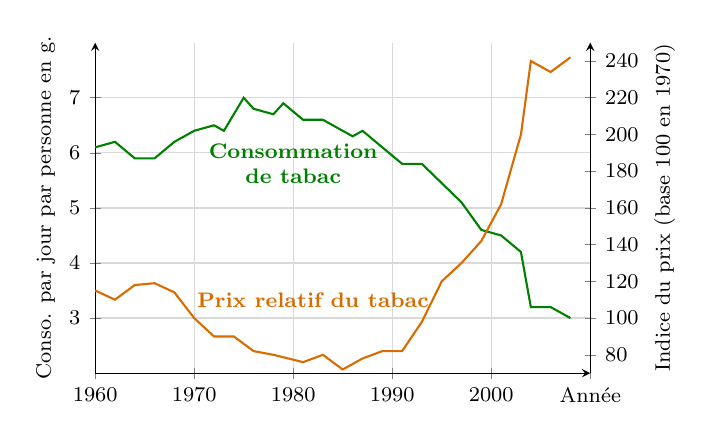
\begin{tikzpicture}[scale=0.95]
			\pgfplotsset{every axis/.append style={ width=8.2cm, height=6cm, xmin=1960, xmax=2010, xtick={1960, 1970, 1980, 1990, 2000, 2010}, xticklabels={1960, 1970, 1980, 1990, 2000, Année}, axis x line=bottom, set layers=standard, tick label style={font=\footnotesize}, cell picture=true, }}
			\begin{axis}[ ymin=2, ymax=8, ytick={3, 4, 5, 6, 7}, axis y line=left, grid=both, grid style={line width=0.5pt, draw=gray!30}, ylabel style={align=center, at={(axis description cs:-0.1,0.5)}, anchor=center, font=\footnotesize}, ylabel={Conso. par jour par personne en g.}, ]
				\addplot[ green!50!black, thick, smooth, tension=0.0 ] coordinates { (1960,6.1) (1962,6.2) (1964,5.9) (1966,5.9) (1968,6.2) (1970,6.4) (1972,6.5) (1973,6.4) (1975,7.0) (1976,6.8) (1978,6.7) (1979,6.9) (1981,6.6) (1983,6.6) (1985,6.4) (1986,6.3) (1987,6.4) (1991,5.8) (1993,5.8) (1997,5.1) (1999,4.6) (2001,4.5) (2003,4.2) (2004,3.2) (2006,3.2) (2008,3.0) };
				\node[green!50!black, font=\footnotesize\bfseries, align=center] at (axis cs:1980,5.8) {Consommation\\de tabac};
			\end{axis}
			\begin{axis}[ ymin=70, ymax=250, ytick={80,100, 120,140, 160, 180,200,220, 240}, axis y line=right, axis x line=none, grid=none, axis background/.style={fill=none}, ylabel style={align=center, at={(axis description cs:1.15,0.5)}, anchor=center, font=\footnotesize}, ylabel={Indice du prix (base $100$ en $1970$)}, ]
				\addplot[ orange!85!black, thick, smooth, tension=0.0 ] coordinates { (1960,115) (1962,110) (1964,118) (1966,119) (1968,114) (1970,100) (1972,90) (1974,90) (1976,82)  (1978,80) (1981,76)  (1983,80)  (1985,72)  (1987,78)  (1989,82) (1991,82)  (1993,98)  (1995,120) (1997,130) (1999,142) (2001,162) (2003,200) (2004,240) (2006,234) (2008,242) };
				\node[orange!85!black, font=\footnotesize\bfseries] at (axis cs:1982,110) {Prix relatif du tabac};
			\end{axis}
		\end{tikzpicture}
	\end{center}

	\begin{enumerate}
		\item Préciser l'année où la consommation de tabac est maximale puis celle où le prix relatif du tabac est minimal.
		\item En considérant, pour simplifier, que la consommation de tabac est croissante puis décroissante, tracer le tableau de variations de la consommation $C$ de tabac en fonction de années $t$.
		\item Procéder de façon analogue pour tracer le tableau de variations du prix $P$ du tabac (pour le minimum, on observera l'année $1985$).
		\item En comparant ces variations, peut-on penser que l'augmentation du prix du tabac a pu faire diminuer la consommation (entre autres facteurs) ?
	\end{enumerate}
\end{exo}
